\documentclass[12pt,a4paper]{article}

\usepackage[top=2.5cm, bottom=2.5cm, left=3cm, right=2.5cm]{geometry}
\usepackage{graphicx}
\usepackage{amsmath, amssymb}
\usepackage{hyperref}
\usepackage{fancyhdr}
\usepackage{setspace}
\usepackage{enumitem}
\usepackage{caption}
\usepackage{float}

\onehalfspacing

\pagestyle{fancy}
\fancyhf{}
\fancyhead[C]{\footnotesize\textit{Deep Learning-Based Vehicle Detection and Traffic Flow Analysis}}
\fancyfoot[C]{\thepage}
\renewcommand{\headrulewidth}{0.4pt}
\renewcommand{\footrulewidth}{0pt}

\fancypagestyle{plain}{
  \fancyhf{}
  \fancyfoot[C]{\thepage}
  \renewcommand{\headrulewidth}{0pt}
}

\begin{document}

% ---- COVER PAGE ----
\begin{titlepage}
\centering
\vspace*{1cm}


\includegraphics[width=4cm]{iust.png}

\vspace{0.8cm}
{\Large\textbf{Iran University of Science and Technology}}\\[0.3cm]
{\large Department of Electrical and Computer Engineering}

\vspace{2cm}
{\large\textsc{Bachelor of Science Thesis}}

\vspace{1.5cm}
{\LARGE\textbf{Deep Learning-Based Vehicle Detection\\[5pt]and Traffic Flow Analysis}}\\[0.3cm]
{\large (Summary)}

\vspace{2cm}
{\large Author}\\[0.3cm]
{\Large\textbf{Ahmadreza Farahani}}

\vspace{1.5cm}
{\large Supervisor}\\[0.3cm]
{\Large\textbf{Prof. Ali Asghar Beheshti}}

\vfill
{\large June 2021\\Tehran, Iran}
\end{titlepage}

% ---- TABLE OF CONTENTS ----
\newpage
\tableofcontents
\newpage

% ---- SECTION 1: OVERVIEW ----
\section{Overview}

This project was developed as part of a national initiative to measure traffic flow through monitoring cameras installed at junctions in Tehran, Iran. The system uses YOLOv4 \cite{yolov4} for vehicle detection, DeepSORT \cite{deepsort} for multi-object tracking, and a semi-supervised approach combining Spectral Clustering \cite{spectral} with SVM \cite{svm} for lane classification.

\textbf{Note:} This project uses YOLOv4 and was trained on limited data with augmentation. Many newer detection and tracking algorithms have since been developed with improved performance.

% ---- SECTION 2: PIPELINE ----
\section{Pipeline}

\subsection{Detection and Tracking}

A custom YOLOv4 model was trained on aerial vehicle imagery. The DeepSORT algorithm \cite{deepsort} handles multi-object tracking using a Kalman filter \cite{kalman} for state prediction and cosine distance for appearance matching.

The tracker maintains vehicle identities across frames using an 8-dimensional state space:

\begin{equation}
\mathbf{x} = [x, y, a, h, \dot{x}, \dot{y}, \dot{a}, \dot{h}]^T
\end{equation}

where $(x, y)$ is the bounding box center, $a$ is the aspect ratio, $h$ is the height, and the remaining components are their respective velocities.

Association between detections and tracks uses a cost matrix combining appearance features (cosine distance) and motion information (Mahalanobis distance), solved via the Hungarian algorithm \cite{hungarian}.

\begin{figure}[H]
\centering
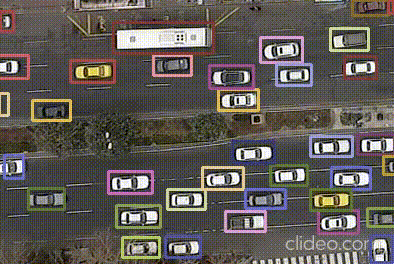
\includegraphics[width=0.85\textwidth]{tracking_frame.png}
\caption{Real-time vehicle detection and tracking using YOLOv4 and DeepSORT.}
\label{fig:tracking}
\end{figure}

\subsection{Lane Clustering}

From tracking, three features are extracted for each detected vehicle and normalized using StandardScaler:

\begin{itemize}[noitemsep]
  \item Horizontal position ($x$)
  \item Vertical position ($y$)
  \item Vehicle angle ($\theta$)
\end{itemize}

Spectral Clustering \cite{spectral} is applied to group vehicles by lane. Processing 1000 frames yielded approximately 60,000 vehicle detections with 180,000 total features. Various clustering algorithms were evaluated using silhouette score, with Spectral Clustering producing the best results.

\begin{figure}[H]
\centering
\includegraphics[width=0.6\textwidth]{spec_4.png}
\caption{Lane clustering using Spectral Clustering with 4 clusters.}
\label{fig:clustering}
\end{figure}

\subsection{SVM Classification}

To refine the clustering results and handle edge cases, an SVM \cite{svm} with RBF kernel was trained on the labeled data from the clustering stage:

\begin{equation}
K(x_i, x_j) = \exp\left(-\gamma \|x_i - x_j\|^2\right)
\end{equation}

The classifier takes normalized $(x, y)$ coordinates and predicts lane assignments, reducing errors in lane boundaries.

\begin{figure}[H]
\centering
\includegraphics[width=0.6\textwidth]{spec_4_svm.png}
\caption{Refined lane classification after SVM training.}
\label{fig:svm}
\end{figure}

\subsection{Real-time Analysis}

The final pipeline integrates all components for real-time video processing. The system classifies each detected vehicle into lanes and calculates per-lane statistics including vehicle count and average speed for traffic management applications.

\begin{figure}[H]
\centering
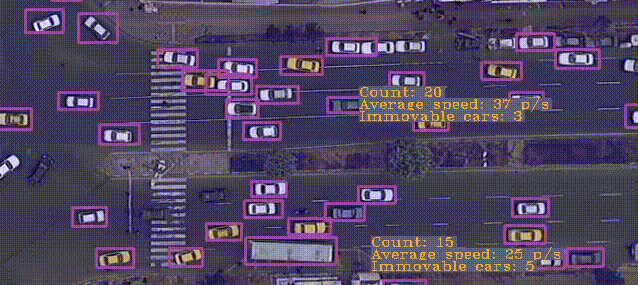
\includegraphics[width=0.85\textwidth]{demo_frame.png}
\caption{Complete pipeline with lane classification and traffic analysis.}
\label{fig:demo}
\end{figure}

% ---- SECTION 3: CONCLUSION ----
\section{Conclusion}

This project demonstrates a complete pipeline for automated traffic flow measurement from aerial imagery. The combination of deep learning-based detection (YOLOv4), robust tracking (DeepSORT with Kalman filtering), and semi-supervised lane classification (Spectral Clustering refined with SVM) provides an automated solution for traffic monitoring at scale.

% ---- REFERENCES ----
\newpage
\begin{thebibliography}{9}

\bibitem{yolov4}
A.~Bochkovskiy, C.-Y.~Wang, and H.-Y.~M.~Liao,
``YOLOv4: Optimal Speed and Accuracy of Object Detection,''
\textit{arXiv preprint arXiv:2004.10934}, 2020.

\bibitem{deepsort}
N.~Wojke, A.~Bewley, and D.~Paschke,
``Simple Online and Realtime Tracking with a Deep Association Metric,''
in \textit{Proc. IEEE International Conference on Image Processing (ICIP)}, 2017.

\bibitem{spectral}
A.~Y.~Ng, M.~I.~Jordan, and Y.~Weiss,
``On Spectral Clustering: Analysis and an Algorithm,''
in \textit{Advances in Neural Information Processing Systems (NeurIPS)}, vol.~14, 2001.

\bibitem{svm}
C.~Cortes and V.~Vapnik,
``Support-Vector Networks,''
\textit{Machine Learning}, vol.~20, no.~3, pp.~273--297, 1995.

\bibitem{hungarian}
H.~W.~Kuhn,
``The Hungarian Method for the Assignment Problem,''
\textit{Naval Research Logistics Quarterly}, vol.~2, no.~1--2, pp.~83--97, 1955.

\bibitem{kalman}
R.~E.~Kalman,
``A New Approach to Linear Filtering and Prediction Problems,''
\textit{Journal of Basic Engineering}, vol.~82, no.~1, pp.~35--45, 1960.

\end{thebibliography}

\end{document}
